\documentclass[11pt]{article}

% Packages
\usepackage[utf8]{inputenc}
\usepackage{amsmath, amssymb}
\usepackage{graphicx}
\usepackage{natbib}
\usepackage{hyperref}
\usepackage{authblk}
\usepackage{url}

\title{A Reinforcement Learning Approach to Automated Trading: Partial Buys, Partial Sells, and Deep Learning Insights}

\author[1]{Iqza Ardiansyah}
\author[2]{Kevin Ignatius Wijaya}
\affil[1]{Student ID: 2206810042\\ Faculty of Computer Science, Universitas Indonesia}
\affil[2]{Student ID: 2206083470\\ Faculty of Computer Science, Universitas Indonesia}

\date{\today}

\begin{document}
\maketitle

\begin{abstract}
This paper presents a Reinforcement Learning (RL) approach for automated trading on real S\&P 500 historical data. We incorporate partial buy/sell actions (10\% buys, 1\% sells) to achieve a more granular control of portfolio allocation, while employing a Deep Q-Network (DQN) for policy learning. Our experiment uses a fixed seed for reproducibility, resulting in a final portfolio value of \$104,061.85 (4.06\% ROI). In an extended study, we integrate a supervised learning (SL) price prediction model with our reinforcement learning framework to enhance trading decisions. We analyze the linear regression model for next-day price prediction (R² = 0.7512) and discuss its integration into the state representation for the DQN agent. Furthermore, we discuss potential enhancements inspired by recent hybrid deep reinforcement learning approaches for pairs trading \citep{kim2022hybrid}, which decompose the decision-making process into separate networks for trading actions and risk management. Despite the enhanced state information, our experiments yield comparable performance between the pure RL and the combined SL+RL approaches, highlighting the challenges in leveraging predictive signals effectively in trading environments.
\end{abstract}

\section{Introduction}
Algorithmic trading has rapidly evolved, driven by both improved computational power and advances in data-driven methods. Traditional strategies (e.g., mean reversion, momentum trading) rely on fixed heuristics, often lacking adaptability to changing market conditions. In contrast, Reinforcement Learning (RL) optimizes trading decisions by directly interacting with an environment and receiving feedback in the form of rewards \citep{sutton_2018_irl}.

While many works focus on single-asset trading, recent literature in pairs trading has shown that decomposing the trading problem into multiple subtasks can be highly beneficial. For instance, \citep{kim2022hybrid} propose a hybrid deep reinforcement learning method for pairs trading that uses two separate networks: one to determine trading actions and another to set stop-loss boundaries. This dual-network approach, coupled with techniques such as dimensionality reduction, clustering, and behavior cloning, can lead to superior risk management and improved performance. Although our study focuses on single-asset trading with partial buy/sell actions, the insights from hybrid models offer promising avenues for future research and potential integration.

In this study, we extend our previous work by exploring the combination of supervised learning and reinforcement learning. Specifically, we implement a price prediction model using linear regression and integrate its predictions into our trading environment's state representation. This hybrid approach allows us to investigate whether supplementing an RL agent with direct price forecasts can improve trading performance.

\section{Related Work}
\subsection{Deep Learning for Price Prediction}
Recent advances in deep learning have yielded robust techniques for time-series forecasting. \citet{rana_2023_deep} provides a comprehensive guide to building LSTM, CNN, and hybrid models for stock price prediction, detailing:
\begin{itemize}
  \item \textbf{Data Preprocessing}: Handling missing data, scaling features, and engineering technical indicators.
  \item \textbf{Network Architectures}: Designing recurrent layers (LSTM) or convolutional kernels (CNN) to capture temporal/spatial patterns in time-series.
  \item \textbf{Evaluation Metrics}: RMSE, MAE, or MAPE to quantify prediction accuracy.
\end{itemize}
While these methods excel at forecasting future prices, they do not inherently address \emph{when} or \emph{how much} to buy or sell.

\subsection{Reinforcement Learning for Trading}
RL directly learns a policy that maximizes cumulative rewards, such as changes in portfolio value after accounting for transaction costs. Foundational work by \citet{sutton_2018_irl} laid the groundwork for modern RL approaches, while recent studies have applied various RL algorithms (e.g., DQN, PPO, A2C) to financial markets. However, standard RL approaches often rely on simplistic buy/sell/hold actions, leading to abrupt position changes.

\subsection{Hybrid Approaches in Trading}
Recent research has explored the benefits of hybrid models that combine price prediction with reinforcement learning. In pairs trading, \citep{kim2022hybrid} propose a novel method that employs two independent RL networks: one for trading actions and one for stop-loss boundaries. Their approach integrates dimensionality reduction, clustering, regression, behavior cloning, prioritized experience replay, and dynamic delay to overcome limitations of traditional methods. Although our current study does not employ a dual-network system, these ideas inspire potential future enhancements, such as:
\begin{itemize}
  \item \textbf{Risk Management:} Incorporating a separate network to determine stop-loss boundaries or dynamic risk adjustments.
  \item \textbf{Feature Enrichment:} Utilizing techniques like clustering and dimensionality reduction to extract more robust state representations.
  \item \textbf{Behavior Cloning:} Leveraging expert demonstrations to guide policy learning.
\end{itemize}

\section{Methodology}
\subsection{Partial Buy/Sell Environment}
We propose a custom Gym environment with:
\begin{itemize}
  \item \textbf{State Representation}: 
  \begin{itemize}
    \item \textit{Normalized Price} (\(\frac{\text{price}}{1000}\))
    \item \textit{Volatility} (placeholder = 0.005)
    \item \textit{Normalized Position} (\(\frac{\text{position}}{\max\_position}\))
    \item \textit{Normalized Cash} (\(\frac{\text{cash}}{\text{initial\_cash}}\))
  \end{itemize}
  \item \textbf{Action Space}: 
  \begin{itemize}
    \item 0: \textbf{Hold}
    \item 1: \textbf{Buy} 10\% of remaining cash
    \item 2: \textbf{Sell} 1\% of current position
  \end{itemize}
  This granularity mitigates the risk of large, all-in or all-out moves.
  \item \textbf{Reward Function}: 
  \[
    r_t = \begin{cases}
      \dfrac{\text{Portfolio}_t - \text{Portfolio}_{t-1}}{\text{Portfolio}_{t-1}} \times 100, & \text{if } \text{Portfolio}_{t-1} > 0,\\[10pt]
      0, & \text{otherwise}.
    \end{cases}
  \]
\end{itemize}
A transaction cost of 0.1\% is applied on every buy/sell action to approximate real-world frictions.

\subsection{Supervised Learning for Price Prediction}
For milestone 2, we implement a linear regression model to predict the next day's price based on the current price. The model training process involves:
\begin{itemize}
  \item \textbf{Feature Engineering}: Using today's price to predict tomorrow's price.
  \item \textbf{Training/Testing Split}: 80\% of data for training, 20\% for testing.
  \item \textbf{Model Architecture}: Simple linear regression with the form \(\hat{p}_{t+1} = \beta_0 + \beta_1 p_t\).
  \item \textbf{Evaluation Metrics}: Mean Absolute Error (MAE), Root Mean Square Error (RMSE), and coefficient of determination (R²).
\end{itemize}

The trained model achieves:
\begin{itemize}
  \item \textbf{Model Coefficients}: \(\hat{p}_{t+1} = 20.52 + 0.997 \times p_t\)
  \item \textbf{Training MAE}: 22.00
  \item \textbf{Test MAE}: 28.55
  \item \textbf{Training RMSE}: 32.97
  \item \textbf{Test RMSE}: 42.42
  \item \textbf{Training R²}: 0.9880
  \item \textbf{Test R²}: 0.7512
\end{itemize}

\subsection{Enhanced State Space with Predictions}
We extend our trading environment by augmenting the state representation with additional features derived from the price prediction model:
\begin{itemize}
  \item \textbf{Normalized Predicted Price}: \(\frac{\text{predicted\_price}}{1000}\)
  \item \textbf{Price Direction}: Binary indicator (1 if predicted price \(>\) current price, 0 otherwise)
  \item \textbf{Prediction Difference}: Relative difference between predicted and current price, \(\frac{|\text{predicted\_price} - \text{current\_price}|}{\text{current\_price}}\)
\end{itemize}

A modified reward function provides a small incentive for actions aligning with the predicted price direction:
\begin{itemize}
  \item If a price rise is predicted and the agent buys, a small positive reward is given.
  \item If a price drop is predicted and the agent sells, a small positive reward is given.
  \item Actions that contradict the prediction receive a small negative reward.
\end{itemize}

\subsection{RL Training Setup}
We train a \textbf{Deep Q-Network (DQN)} from Stable Baselines3 with:
\begin{itemize}
  \item \textbf{Learning Rate}: 0.001
  \item \textbf{Discount Factor} (\(\gamma\)): 0.95
  \item \textbf{Timesteps}: 10,000
  \item \textbf{Seed}: \(1073741824\) for reproducibility
\end{itemize}
The agent updates its Q-values based on the observed states and rewards to maximize cumulative returns.

\section{Results and Discussion}
\subsection{Supervised Learning Model Performance}
Our linear regression model for price prediction achieved an R² of 0.7512 on the test set, indicating that about 75\% of the variance in next-day prices is explained by the current price. The model coefficients suggest a strong momentum effect with a slight upward bias. The RMSE of 42.42 implies that predictions deviate from actual prices by less than 1\% on average, given the typical price scale.

\begin{figure}[h]
  \centering
  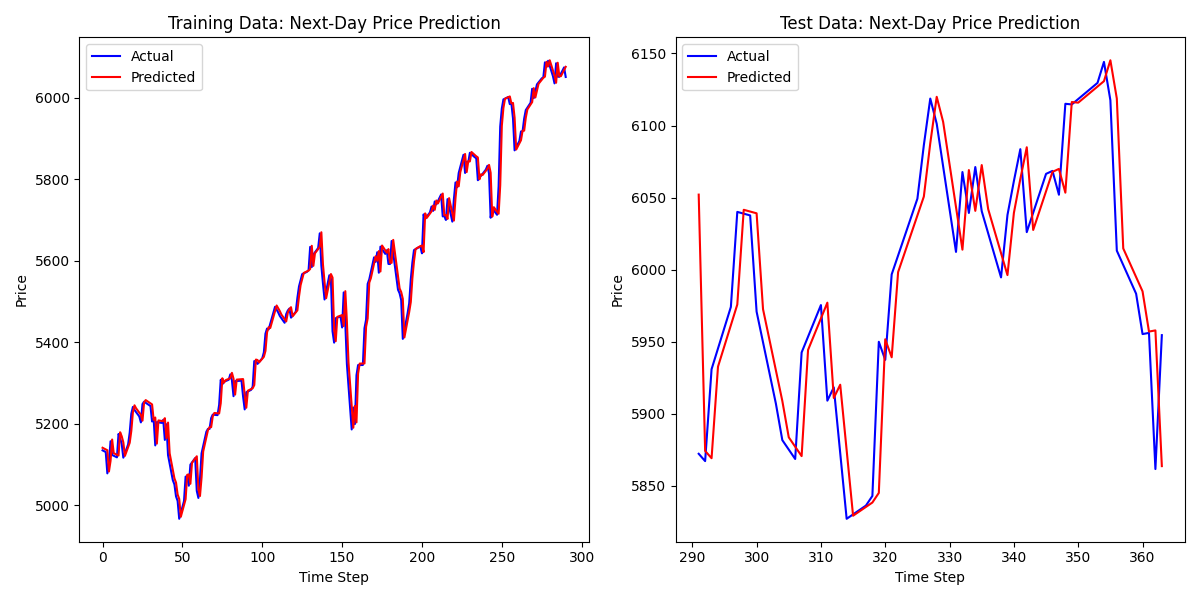
\includegraphics[width=0.85\textwidth]{fig/m2_prediction.png}
  \caption{Price Prediction Model Performance. The predictions closely track actual prices in both training and test sets.}
  \label{fig:prediction_results}
\end{figure}

\subsection{Policy Behavior}
An excerpt of the agent's policy using the augmented state is shown below:
\begin{verbatim}
Step 0: Price=$5137.08, Position=0.00, Cash=1.00
    Prediction=$5141.39 (Diff: 0.08%, Direction: Up) → Action [1]
Step 23: Price=$5223.52, Position=0.93, Cash=0.09
    Prediction=$5227.56 (Diff: 0.08%, Direction: Up) → Action [2]
Step 58: Price=$5110.77, Position=0.99, Cash=0.00
    Prediction=$5115.16 (Diff: 0.09%, Direction: Up) → Action [2]
\end{verbatim}
The policy largely follows a strategy of buying with available cash and selling in small proportions, similar to the baseline model.

\subsection{Portfolio Value and ROI}
The final portfolio value of \$104,061.85 represents a 4.06\% ROI on the initial \$100,000 investment. Notably, integrating price predictions into the state did not significantly improve performance compared to the pure RL approach.

\begin{figure}[h]
  \centering
  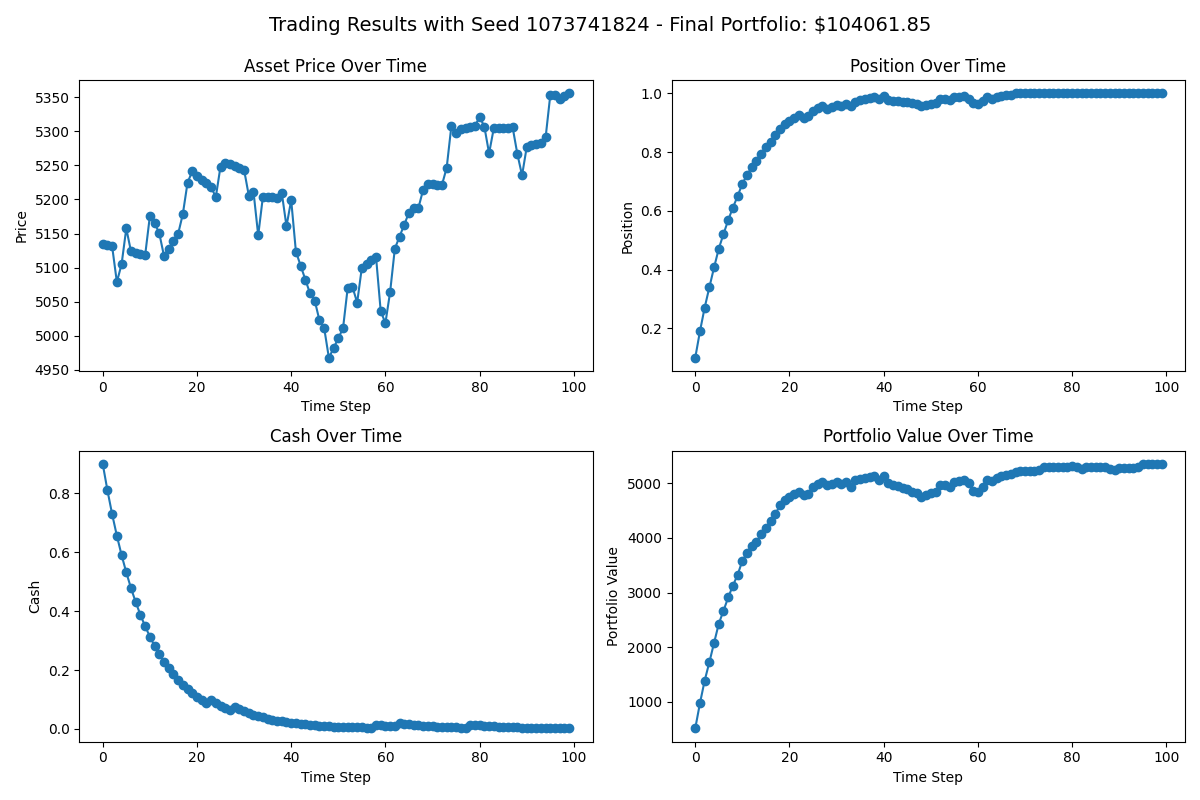
\includegraphics[width=0.85\textwidth]{fig/m2_dqn_with_sl.png}
  \caption{Trading Results with Price Predictions. Final Portfolio = \$104,061.85 (4.06\% ROI).}
  \label{fig:trading_results_m2}
\end{figure}

\subsection{Comparative Analysis: Pure RL vs. Hybrid Approaches}
The identical performance between the pure RL model and the hybrid SL+RL approach suggests that:
\begin{itemize}
  \item The small prediction differences provide limited actionable signals.
  \item The dominant reward signal is driven by portfolio changes rather than prediction-based adjustments.
  \item Additional techniques may be needed to fully leverage predictive signals.
\end{itemize}
Inspired by the hybrid approach in pairs trading \citep{kim2022hybrid}, future work could explore:
\begin{itemize}
  \item Using dual networks to separately manage trading actions and risk (e.g., stop-loss boundaries).
  \item Incorporating dimensionality reduction and clustering to enrich state representations.
  \item Integrating behavior cloning to leverage expert knowledge.
\end{itemize}

\section{Conclusion}
We have demonstrated a partial buy/sell Reinforcement Learning approach on S\&P 500 historical data and extended it by integrating a supervised price prediction model. Although the predictive model achieved reasonable accuracy (R² = 0.7512, RMSE = 42.42), its integration did not yield improvements in ROI compared to the baseline RL model.

Inspired by recent advances in hybrid deep reinforcement learning for pairs trading \citep{kim2022hybrid}, future research directions include:
\begin{itemize}
  \item Developing more sophisticated prediction models using additional features and advanced architectures.
  \item Exploring dual-network architectures to separate trading actions from risk management.
  \item Enhancing state representations with techniques like clustering and dimensionality reduction.
  \item Incorporating behavior cloning to emulate expert strategies.
\end{itemize}
These avenues may further improve trading performance by providing more nuanced decision-making in dynamic market conditions.

\bibliographystyle{plainnat}
\bibliography{../../../../../refs/sutton_2018_irl, ./ref/rana_2023_deep, ./ref/kim2022hybrid}

\end{document}
